\documentclass[executivepaper]{article}

\usepackage{graphicx}
\usepackage[utf8]{inputenc}
\usepackage[T1]{fontenc}
\usepackage[spanish]{babel} % Establece el idioma español
\usepackage{csquotes} % Carga el paquete csquotes
\usepackage{graphicx} % Required for inserting images
\usepackage{listings}
\usepackage{xcolor}
\usepackage{hyperref}
\usepackage[left=1.00cm, right=1.00cm, top=2.00cm, bottom=2.00cm]{geometry}
\usepackage{tikz}
\usetikzlibrary{shapes,arrows}
\usetikzlibrary{positioning}
\setlength{\parindent}{0.5in}
\usepackage{setspace}
\doublespacing

\lstset{
    inputencoding=utf8,
    language=Java,
    basicstyle=\ttfamily,
    columns=fullflexible
}

% Define colores para el código
\definecolor{codegreen}{rgb}{0,0.6,0}
\definecolor{codegray}{rgb}{0.5,0.5,0.5}
\definecolor{codepurple}{rgb}{0.58,0,0.82}
\definecolor{backcolour}{rgb}{0.95,0.95,0.92}

% Configuración de lstlisting
\lstdefinestyle{mystyle}{
    backgroundcolor=\color{backcolour},   
    commentstyle=\color{codegreen},
    keywordstyle=\color{magenta},
    numberstyle=\tiny\color{codegray},
    stringstyle=\color{codepurple},
    basicstyle=\ttfamily\footnotesize,
    breakatwhitespace=false,         
    breaklines=true,                 
    captionpos=b,                    
    keepspaces=true,                 
    numbers=left,                    
    numbersep=5pt,                  
    showspaces=false,                
    showstringspaces=false,
    showtabs=false,                  
    tabsize=2
}

% Configuración del paquete hyperref
\hypersetup{
    colorlinks=true,
    linkcolor=black,
    filecolor=magenta,      
    urlcolor=gray,
}

\lstset{style=mystyle}

\title{Informe sobre JAVA}
\author{Kevin Cárdenas}

\begin{document}

\begin{titlepage}
    \begin{center}
        {\Huge \textbf{Programación orientada a objetos}}
        \\[18cm]

        \large\emph{Autor:}\\
        Kevin Cárdenas.
        \\[1cm]
        {\large 2023}
    \end{center}
\end{titlepage}

\newpage
\tableofcontents
\newpage
\section{Introducción}
La programación orientada a objetos (\enquote*{POO}) es un paradigma de programación que se enfoca en la creación de objetos que contienen tanto datos como funciones que actúan sobre esos datos. Esta técnica de programación se centra en la creación de \textit{clases} que definen los objetos, y los objetos son instancias de esas clases.

En POO, los objetos son considerados como \enquote*{cosas} que tienen ciertas propiedades y comportamientos. Cada objeto puede tener un conjunto de datos asociados (denominados \enquote*{atributos} o \enquote*{propiedades}), así como una serie de funciones o \enquote*{métodos} que pueden realizar acciones sobre esos datos.

Una de las principales ventajas de la POO es que permite la modularidad del código, lo que significa que puedes dividir el código en pequeñas secciones que se pueden desarrollar, probar y mantener de forma independiente. Además, la POO también hace que el código sea más fácil de entender y mantener a largo plazo, ya que las funciones y datos relacionados están agrupados en objetos que tienen un propósito claro.

\subsection{Encapsulación, Herencia, Polimorfismo y Abstracción}
En POO, hay cuatro conceptos fundamentales que se deben entender:
\begin{enumerate}
    \item \textit{Encapsulación}: este concepto se refiere a la ocultación de datos y métodos dentro de un objeto para que solo puedan ser accedidos por el objeto mismo o por otros objetos que tengan una relación específica con él.
    \item \textit{Herencia}: la herencia permite crear una clase nueva a partir de una ya existente, pero añadiéndole o modificando sus propiedades y métodos.
    \item \textit{Polimorfismo}: este concepto se refiere a la capacidad de diferentes objetos de una misma clase para responder de manera distinta a un mismo mensaje o función.
    \item \textit{Abstracción}: la abstracción se refiere a la capacidad de crear una clase que representa un concepto o idea abstracta, sin necesidad de especificar todos los detalles en su definición.
\end{enumerate}
La POO se utiliza en muchos lenguajes de programación populares, como Java, Python, C++ y muchos otros

\subsection*{JAVA orientado a objetos}
Java es uno de los lenguajes de programación más populares y utilizados en el mundo, y también es conocido por su fuerte orientación a objetos. En Java, todo es un objeto, incluso los tipos primitivos, como los enteros y los caracteres, se representan como objetos.

La POO en Java se basa en la definición de clases y objetos. Una \textit{clase} es un plano o plantilla que define la estructura, atributos y métodos de los objetos que se pueden crear a partir de ella. Un \textit{objeto} es una instancia de una clase, es decir, un miembro concreto de la clase que contiene sus propios valores para los atributos definidos en la clase.

La encapsulación en Java se logra mediante el uso de modificadores de acceso, como \texttt{private}, \texttt{protected} y \texttt{public}, que permiten controlar el acceso a los atributos y métodos de una clase desde otras clases. La herencia se logra mediante la extensión de una clase existente mediante la palabra clave \texttt{extends}. El polimorfismo se logra mediante la implementación de interfaces o mediante la sobrecarga y la anulación de métodos.

La abstracción en Java se logra mediante el uso de interfaces y clases abstractas. Una \textit{interface} es una colección de métodos sin implementación que una clase puede implementar para proporcionar su propia implementación. Una \textit{clase abstracta} es una clase que no se puede instanciar directamente, sino que debe ser subclasificada y extendida.

\subsection*{Python orientado a objetos}
Python es un lenguaje de programación de alto nivel y fácil de aprender que también es conocido por su fuerte orientación a objetos. En Python, todo es un objeto, desde los números y las cadenas hasta las funciones y las clases.

La POO en Python se basa en la definición de clases y objetos. Una \textit{clase} es un plano o plantilla que define la estructura, atributos y métodos de los objetos que se pueden crear a partir de ella. Un \textit{objeto} es una instancia de una clase, es decir, un miembro concreto de la clase que contiene sus propios valores para los atributos definidos en la clase.

La encapsulación en Python se logra mediante el uso de convenciones de nomenclatura, como el uso de guiones bajos (\lstinline{_}) o doble guiones bajos (\lstinline{__}) para indicar la visibilidad de los atributos y métodos. La herencia se logra mediante la herencia de una clase existente mediante la palabra clave \lstinline{class ClassName(ParentClass)}. El polimorfismo se logra mediante la implementación de métodos con el mismo nombre en diferentes clases.

La abstracción en Python se logra mediante el uso de clases abstractas y métodos abstractos. Una \textit{clase abstracta} es una clase que no se puede instanciar directamente, sino que debe ser subclasificada y extendida. Un \textit{método abstracto} es un método que se define en una clase abstracta pero no se implementa, lo que significa que las subclases deben proporcionar su propia implementación.

Python también es conocido por su soporte para la programación orientada a objetos basada en funciones. En este enfoque, las funciones se utilizan para encapsular la lógica de la clase y para proporcionar una interfaz más clara para el uso de la clase.

\subsection{Modelado}
El modelado es una parte fundamental de la programación orientada a objetos. El objetivo del modelado es crear un modelo conceptual de un sistema o aplicación en términos de clases, objetos, atributos, métodos y relaciones entre ellos.

En el modelado, se utilizan diagramas de clases para representar la estructura de un sistema. Un diagrama de clases es una representación gráfica de las clases en un sistema y las relaciones entre ellas. Las clases se representan como cajas con el nombre de la clase, sus atributos y métodos. Las relaciones entre las clases se representan mediante líneas que indican la naturaleza de la relación.

Además de los diagramas de clases, también se utilizan otros diagramas para modelar otros aspectos de la programación orientada a objetos. Por ejemplo, el diagrama de secuencia se utiliza para modelar la interacción entre objetos en un sistema, el diagrama de estado se utiliza para modelar el comportamiento de un objeto en diferentes estados y el diagrama de actividades se utiliza para modelar el flujo de trabajo de un proceso.

El modelado es una parte importante del desarrollo de software orientado a objetos porque ayuda a los desarrolladores a comprender mejor el sistema que están construyendo y a identificar y resolver problemas potenciales antes de escribir cualquier código. También ayuda a garantizar que el sistema sea modular, fácil de entender y mantener a largo plazo.

\subsection*{UML - Lenguaje de Modelado Unificado}
UML (\enquote*{Lenguaje de Modelado Unificado}) es un lenguaje de modelado visual utilizado para el diseño y la documentación de sistemas de software orientados a objetos. UML es una herramienta popular utilizada por los desarrolladores de software para visualizar, especificar, construir y documentar los sistemas de software.

El lenguaje UML consta de varios tipos de diagramas, cada uno de los cuales se utiliza para modelar diferentes aspectos de un sistema de software. Estos diagramas incluyen:

\begin{enumerate}
\item Diagrama de Clases: representa la estructura estática del sistema, incluyendo las clases, los atributos y los métodos, y las relaciones entre ellos.
\item Diagrama de Objetos: representa una instancia específica de una clase en un punto específico del tiempo, incluyendo los valores de los atributos.
\item Diagrama de Casos de Uso: representa los actores, los casos de uso y las relaciones entre ellos.
\item Diagrama de Secuencia: representa la interacción entre los objetos en una secuencia de eventos.
\item Diagrama de Actividad: representa el flujo de trabajo de un proceso o algoritmo.
\item Diagrama de Estados: representa el comportamiento de un objeto en diferentes estados.
\item Diagrama de Componentes: representa los componentes del sistema y las relaciones entre ellos.
\item Diagrama de Despliegue: representa la distribución física del sistema en el hardware.
\end{enumerate}

Estos diagramas son útiles para modelar diferentes aspectos de un sistema de software y proporcionan una visión completa del sistema desde diferentes perspectivas. Los diagramas de UML son útiles tanto para los desarrolladores como para los interesados en el sistema, como los gerentes de proyecto y los clientes, ya que proporcionan una visión clara y detallada del sistema.

\subsubsection*{Clases}
Las clases se representan así:\\
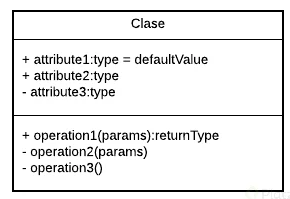
\includegraphics[scale=0.5]{2.1.png}\\
En la parte superior se colocan los atributos o propiedades, y debajo las operaciones de la clase. Notarás que el primer caracter con el que empiezan es un símbolo. Este denotará la visibilidad del atributo o método, esto es un término que tiene que ver con Encapsulamiento y veremos más adelante a detalle.\\
Estos son los niveles de visibilidad que puedes tener:
\begin{enumerate}
    \item $-$  private
    \item $+$  public
    \item $\#$  protected
    \item $~$  default
\end{enumerate}

Una forma de representar las relaciones que tendrá un elemento con otro es a través de las flechas en UML, y aquí tenemos varios tipos, estos son los más comunes:
\subsubsection*{Asociación}
Como su nombre lo dice, notarás que cada vez que esté referenciada este tipo de flecha significará que ese elemento contiene al otro en su definición.\\
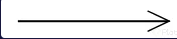
\includegraphics[scale=0.5]{2.2.png}\\
La flecha apuntará hacia la dependencia.\\
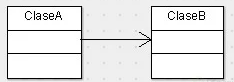
\includegraphics[scale=0.5]{2.3.png}\\
Con esto vemos que la ClaseA está asociada y depende de la ClaseB.
\subsubsection*{Herencia}
Siempre que veamos este tipo de flecha se estará expresando la herencia.\\
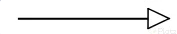
\includegraphics[scale=0.5]{2.4.png}\\
La dirección de la flecha irá desde el hijo hasta el padre.\\
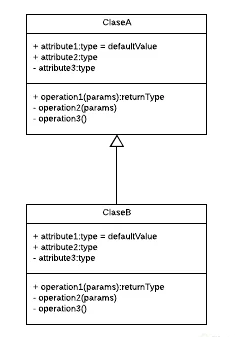
\includegraphics[scale=0.5]{2.5.png}\\
Con esto vemos que la ClaseB hereda de la ClaseA
\subsubsection*{Agregación}
Este se parece a la asociación en que un elemento dependerá del otro, pero en este caso será: Un elemento dependerá de muchos otros.\\
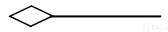
\includegraphics[scale=0.5]{2.6.png}\\
Aquí tomamos como referencia la multiplicidad del elemento. Lo que comúnmente conocerías en Bases de Datos como Relaciones uno a muchos.\\
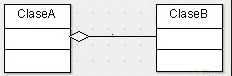
\includegraphics[scale=0.5]{2.7.png}\\
Con esto decimos que la ClaseA contiene varios elementos de la ClaseB. Estos últimos son comúnmente representados con listas o colecciones de datos.
\subsubsection*{Composición}
Este es similar al anterior solo que su relación es totalmente compenetrada.\\
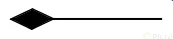
\includegraphics[scale=0.5]{2.8.png}\\
De tal modo que conceptualmente una de estas clases no podría vivir si no existiera la otra.\\
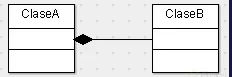
\includegraphics[scale=0.5]{2.9.png}\\

\subsection{Buenas practicas}
Aquí hay algunas buenas prácticas a seguir al trabajar con programación orientada a objetos:
\begin{enumerate}
    \item Utilizar la encapsulación: La encapsulación es una técnica que ayuda a ocultar los detalles de implementación de una clase y permite que los objetos interactúen entre sí solo a través de interfaces definidas. Esto ayuda a reducir el acoplamiento y hace que el código sea más fácil de mantener.
    \item Diseñar clases cohesivas: Una clase cohesiva es aquella que tiene una única responsabilidad claramente definida y no hace más de lo que se espera de ella. Al diseñar clases cohesivas, se reduce la complejidad del código y se facilita la comprensión y el mantenimiento.
    \item Utilizar la herencia con precaución: La herencia es una técnica útil para compartir código común entre clases relacionadas. Sin embargo, se debe tener cuidado al usarla para evitar la creación de clases altamente acopladas y difíciles de mantener.
    \item Evitar la duplicación de código: La duplicación de código puede llevar a errores y dificultar el mantenimiento. Por lo tanto, se deben buscar formas de reutilizar el código existente y evitar la duplicación innecesaria
    \item Mantener el código limpio y legible: Un código limpio y legible es más fácil de entender, mantener y escalar. Se deben seguir buenas prácticas de codificación, como nombrar variables y métodos de manera descriptiva, utilizar comentarios y espacios en blanco adecuados, y seguir un estilo de codificación consistente en todo el proyecto.
    \item Seguir los principios SOLID: Los principios SOLID son un conjunto de reglas que ayudan a garantizar que el código sea fácil de entender, mantener y escalar. Estos principios incluyen la responsabilidad única, la abstracción, la inversión de dependencias, la sustitución de Liskov y la segregación de interfaces.

    los principios SOLID: Los principios SOLID son un conjunto de reglas que ayudan a garantizar que el código sea fácil de entender, mantener y escalar. Estos principios incluyen la responsabilidad única, la abstracción, la inversión de dependencias, la sustitución de Liskov y la segregación de interfaces.
    \begin{itemize}
        \item Principio de responsabilidad única (SRP): Cada clase o módulo debe tener una sola responsabilidad. Esto significa que la clase o módulo debe tener una sola razón para cambiar. Si una clase o módulo tiene más de una responsabilidad, es más difícil de entender y mantener.
        \item Principio de abierto/cerrado (OCP): Las clases o módulos deben estar abiertos para su extensión, pero cerrados para su modificación. Esto significa que si necesitamos agregar una nueva funcionalidad, debemos hacerlo a través de la extensión del código existente, en lugar de modificarlo directamente.
        \item Principio de sustitución de Liskov (LSP): Las clases derivadas deben ser sustituibles por sus clases base. Esto significa que una instancia de una clase derivada debe ser capaz de ser usada en cualquier lugar donde se espera una instancia de la clase base, sin que se produzcan errores o comportamientos inesperados.
        \item Principio de segregación de la interfaz (ISP): Los clientes no deben ser obligados a depender de interfaces que no usan. Esto significa que una clase o módulo no debería tener que depender de métodos o interfaces que no necesita.
        \item Principio de inversión de dependencia (DIP): Las clases de alto nivel no deben depender de las clases de bajo nivel. Ambas clases deben depender de abstracciones. Esto significa que el código de alto nivel no debería depender directamente del código de bajo nivel, sino de una interfaz o abstracción que encapsule el comportamiento del código de bajo nivel.
    \end{itemize}
\end{enumerate}

\subsection{Metodo constructor}
En programación orientada a objetos, un constructor es un método especial utilizado para inicializar un objeto recién creado una vez que se ha reservado memoria para él. El constructor se llama automáticamente al crear un objeto y es responsable de asignar valores iniciales a los atributos de la clase. En Java, el constructor se define con el nombre de la clase y no tiene tipo de retorno.

A continuación, se muestra un ejemplo de un constructor en Java:

\begin{lstlisting}[language=Java]
public class Persona {
    private String nombre;
    private int edad;
    private String direccion;
    
    public Persona(String nombre, int edad, String direccion) {
        this.nombre = nombre;
        this.edad = edad;
        this.direccion = direccion;
    }
    
    // metodos getters y setters
    
    public static void main(String[] args) {
        Persona persona = new Persona("Juan", 30, "Calle 123, Ciudad");
        
        System.out.println("Nombre: " + persona.getNombre());
        System.out.println("Edad: " + persona.getEdad());
        System.out.println("Direccion: " + persona.getDireccion());
        
        persona.setEdad(31);
        System.out.println("Nueva edad: " + persona.getEdad());
    }
}
\end{lstlisting}
En este ejemplo, la clase Persona tiene tres atributos: nombre, edad y direccion. Además, tiene un constructor que recibe estos tres parámetros y los asigna a los atributos correspondientes.

En el método main, se crea una instancia de la clase Persona utilizando el constructor que recibe los valores "Juan", 30 y "Calle 123, Ciudad". Luego, se imprimen los valores de los atributos utilizando los métodos getters correspondientes. Finalmente, se modifica la edad utilizando el método setter correspondiente y se vuelve a imprimir el valor de la edad para verificar que se ha modificado correctamente.

Te presento el ejemplo de un método constructor en Python:
\begin{lstlisting}[language=Python]
class Persona:
    def __init__(self, nombre, edad, direccion):
        self.nombre = nombre
        self.edad = edad
        self.direccion = direccion

    def get_nombre(self):
        return self.nombre

    def set_nombre(self, nombre):
        self.nombre = nombre

    def get_edad(self):
        return self.edad

    def set_edad(self, edad):
        self.edad = edad

    def get_direccion(self):
        return self.direccion

    def set_direccion(self, direccion):
        self.direccion = direccion


# Creamos una instancia de la clase Persona
persona = Persona("Juan", 30, "Calle 123, Ciudad")

# Accedemos a los atributos y metodos de la instancia
print("Nombre: ", persona.get_nombre())
print("Edad: ", persona.get_edad())
print("Direccion: ", persona.get_direccion())

# Modificamos la edad de la persona
persona.set_edad(31)

# Volvemos a imprimir los atributos de la instancia
print("Nueva edad: ", persona.get_edad())
\end{lstlisting}
En este ejemplo, creamos la clase \enquote*{Persona} con un método constructor \lstinline{__init__} que inicializa los atributos de la clase con los valores proporcionados al crear una instancia de la clase. También definimos los métodos get y set para acceder y modificar los atributos de la clase.

Luego, creamos una instancia de la clase \enquote*{Persona} con el nombre \enquote*{Juan}, la edad 30 y la dirección \enquote*{Calle 123, Ciudad}. Accedemos a los atributos y métodos de la instancia para imprimir su información y modificar su edad.

\newpage
\section{JAVA orientada a objetos}
Java es un lenguaje de programación orientado a objetos (POO) que se ha convertido en uno de los más populares en la actualidad. Su éxito se debe en gran medida a su capacidad para manejar de manera eficiente la programación orientada a objetos. 
\subsection{Clase}
Definamos una clase, el formato es el siguiente:
\begin{lstlisting}
public class Person {
    String name = ""
    void walk(){

    }
}
\end{lstlisting}
Este fregmento define una clase llamada \enquote*{Person} que tiene un atributo \enquote*{name} de tipo String y un método \enquote*{walk} que no hace nada.

Por ejemplo:
\begin{lstlisting}
public class Persona {
    private String nombre;
    private int edad;
    private String direccion;

    public Persona(String nombre, int edad, String direccion) {
        this.nombre = nombre;
        this.edad = edad;
        this.direccion = direccion;
    }

    public String getNombre() {
        return nombre;
    }

    public void setNombre(String nombre) {
        this.nombre = nombre;
    }

    public int getEdad() {
        return edad;
    }

    public void setEdad(int edad) {
        this.edad = edad;
    }

    public String getDireccion() {
        return direccion;
    }

    public void setDireccion(String direccion) {
        this.direccion = direccion;
    }
}
    
\end{lstlisting}
Este es un ejemplo de una clase \enquote*{Persona} que tiene tres atributos privados (nombre, edad y dirección) y los métodos públicos necesarios para acceder y modificar estos atributos.

En la línea 1, se define la clase pública \enquote*{Persona}. Los atributos \enquote*{nombre}, \enquote*{edad} y \enquote*{direccion} son definidos en las líneas 2-4 como variables de tipo privado para protegerlos de accesos no deseados.

A continuación, se define el constructor de la clase en las líneas 6-10. Este constructor tiene tres parámetros (nombre, edad y dirección) y se utiliza para crear una nueva instancia de la clase \enquote*{Persona}. Dentro del constructor, se inicializan los atributos de la clase con los valores recibidos en los parámetros utilizando la palabra clave \enquote*{this}.

Luego, se definen los métodos \enquote*{get} y \enquote*{set} para acceder y modificar los valores de los atributos de la clase en las líneas 12-29. Cada método \enquote*{get} devuelve el valor correspondiente del atributo, mientras que cada método \enquote*{set} actualiza el valor del atributo con el valor proporcionado como parámetro.

Por último, se define el método \enquote*{main} en las líneas 31-38. Este es el punto de entrada del programa y se utiliza para crear una instancia de la clase \enquote*{Persona} con valores iniciales y para imprimir los valores de los atributos utilizando los métodos \enquote*{get}. También se utiliza el método \enquote*{setEdad} para actualizar la edad de la persona y se vuelve a imprimir para confirmar que el valor ha sido actualizado correctamente.


\newpage
\section{Python orientado a objetos}
\subsection{Clase}
\begin{lstlisting}[language=Python]
class Person:
    String name = ""
    void walk():

\end{lstlisting}
Este fregmento define una clase llamada "Person" que tiene un atributo "name" de tipo String y un método "walk" que no hace nada.

\newpage
\section{Bibliografía}
\begin{thebibliography}{9}
\bibitem{clean-code} Martin, Robert C. \textit{Clean Code: A Handbook of Agile Software Craftsmanship}. Prentice Hall, 2008.
\bibitem{platzi-java-basico} Platzi. \textit{Curso de Java Básico}. Platzi, 2023.\\ \url{https://platzi.com/cursos/java-basico/}
\bibitem{platzi-java-oo} Platzi. \textit{Curso de Java Orientado a Objetos}. Platzi, 2023.\\ \url{https://platzi.com/cursos/java-poo/}
\bibitem{java-docs} Oracle Corporation. \textit{Java SE Documentation}. Oracle Corporation, 2023.\\ \url{https://docs.oracle.com/en/java/javase/index.html}
\end{thebibliography}



\end{document}